%Include prior work here (i.e. Juan and Akua's)
%----------| section  outline |----------%
\subsection{The Piece-wise Constant-Curvature Model} \label{pccmodeldef}
It was mentioned earlier that in the formulation of the dynamical model to develop a controller around, towing the balance between mathematical simplicity and physical accuracy is one of the major challenges in model-based controls. While this continues to be true, continuum dynamics-compatible FDM techniques has also indeed broken considerable ground regarding this issue. In their exact formulation, the dynamics of a soft robot is effectively an infinite-dimensional system. Such a system cannot be described without the use of partial differential equations (PDEs). However, by applying the appropriate assumptions, approximations, and/or discretization to the dynamical model of the soft robot, the system's description may be reliably "minimized" into a \textit{finite}-dimensional system that can be described with ordinary differential equations (ODEs) instead.

One of the most widely-implemented family of FDM techniques is the Piece-wise Constant Strain (PCS) approximations (see \autoref{rodandpcs}). It is a family of discretization methods applied to a type of approximation for soft robot dynamics known as "rod models". It is extremely common for soft robots to be "thin" and/or "elongated": to have one physical dimension dominate the other two. In that regard, such soft robots may be approximated as a rod with the continuum mechanics of one too--hence rod models. At the heart of this methodology is the assumption that volumetric deformations may be neglected, and modeling the dynamics around the dominant central axis is sufficient \cite{della_santina_model-based_2023}.

\begin{figure}[h!]
    \centering
    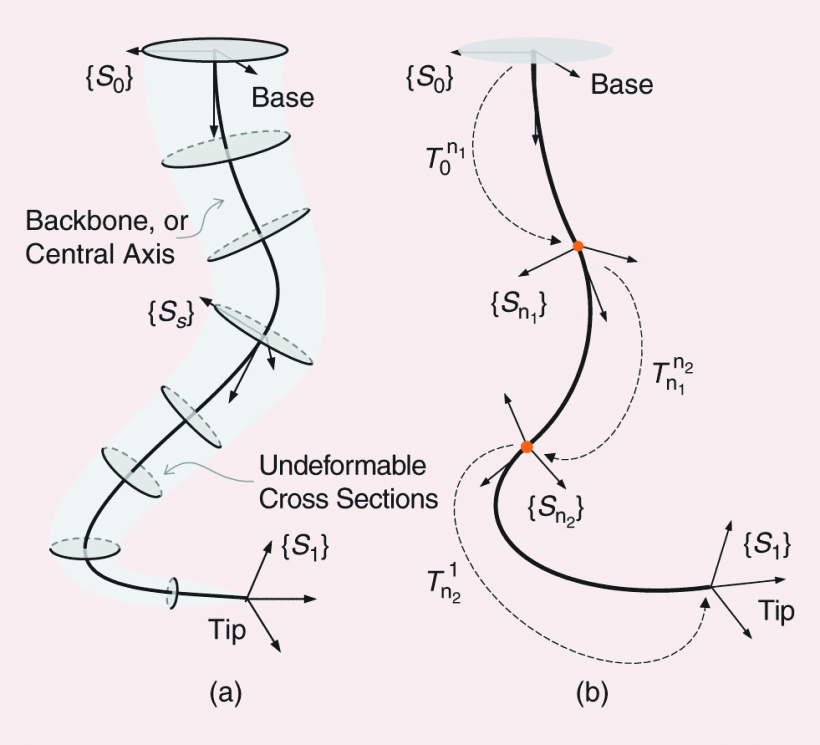
\includegraphics[width=0.6\textwidth]{graphics/roddiagram.png}
    \caption{a) "Elongated" soft robots as described in rod models. b) PCS discretization applied to the rod model. \imgcite{della_santina_model-based_2023}}
    \label{rodandpcs}
\end{figure}

Among the many implementations of PCS, the planar Piece-wise Constant Curvature (PCC) model has been extensively used in soft robotics throughout the last decade. Its approximation of the robot as pieces of constant-curvature arcs linked together in series with mutually tangent connection points makes the kinematics and Jacobian formulation for the model \textit{closed}-form \cite{websteriii_design_2010}. A dynamic feedback controller using this model was developed in \cite{della_santina_model-based_2020}, with an implementation of a trajectory generator for the controller formulated in \cite{dickson_real-time_2025}. 

There are many viable models out there that can be used as the basis for the controller that this proposed thesis seeks to develop, a selection of them that seems promising with respect to the scope of this proposed thesis is outlined below.
%----------| 1. CD Santina's 2020 paper, AND Akua+Juan's subsequent traj. gen. paper for it
\subsection{PCC in an Augmented Rigid Body Model} \label{augmentedpccdef}
The controller from \cite{della_santina_model-based_2020} mentioned earlier uses the kinematics of PCC matched to the dynamics of an augmented rigid body, allowing control strategies typically implemented for rigid-body robots to be used in this scenario. This augmented formulation was initially proposed in \cite{della_santina_dynamic_2018} by Della Santina et al. as well. 

Recall that the PCC Model essentially approximates a rod-like soft robot as a series of constant-curvature (CC) arc segments with mutually-tangent connections. Della Santina et al. proposed that for a given CC segment, the dynamics of the segment can be matched to a rigid-robotic structure comprised of Revolute-Prismatic-Prismatic-Revolute (RPPR) joints in series (see \autoref{pccrigid}). A point mass is located between the two prismatic joints and also matched to the CC segment's center of mass, ensuring the inertial properties of the rigid robot matches the CC segment \cite{della_santina_dynamic_2018}.

\begin{figure}[!h]
    \centering
    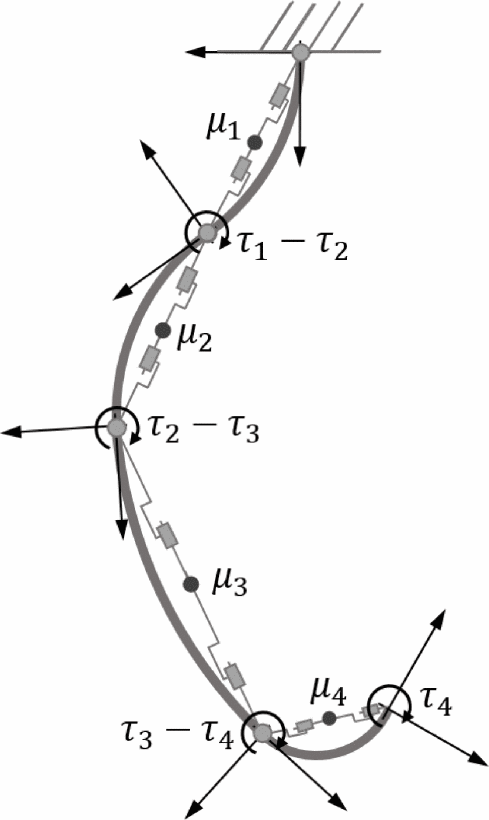
\includegraphics[width=0.3\textwidth]{graphics/pccrigid.png}
    \caption{A series of CC Segments matched to a series of RPPR Robots. \imgcite{della_santina_dynamic_2018}}
    \label{pccrigid}
\end{figure}

Using this model, Della Santina et al. were able to develop two feedback controllers aimed at different implementations. The first controller is intended for trajectory tracking, while the second for Cartesian impedance control. While the model \textit{and} controller does not cover three-dimensional motion, preliminary work into translating the model to three-dimensions is explored in \cite{katzschmann_dynamic_2019}. Implementing this "augmented rigid body" model for this proposed thesis will involve expanding the preliminary work into the three-dimensional translation of the model, and then implementing the control design methodology already laid out in \cite{della_santina_model-based_2020}. The body of literature available to build on regarding this model is one of the biggest appeals in using it for this proposed thesis. However, the kinematic singularity found in the three-dimensional straight configuration remains a challenge.
%----------| 2. CD Santina's subsequent 2020 paper on Arc-Length parametrization for PCC
\subsection{PCC Using an Alternative State Parametrization} \label{altpccdef}
Another one of Cosimo Della Santina's works using the PCC model can be found in \cite{della_santina_improved_2020}. In this work, Della Santina et al. proposes an \textit{alternative} state parametrization for PCC kinematics that describes the CC segments based on the arc lengths of four arcs that bound the surface of the segment.

In the preliminary work of \cite{katzschmann_dynamic_2019}, the PCC kinematics of a soft robot were parametrized according to \autoref{oldparam}. In \cite{della_santina_improved_2020}, Della Santina et al. refers to this state parametrization as the "$\alpha$-parametrization". Kinematically speaking, the $\alpha$-parametrization is defined as $\alpha_i = [\phi_i, \theta_i,\delta L_i]^T$ for the $i$-th CC segment, where $\alpha_i \in \mathbb{R}^3$. In this parametrization, $\phi_i$ and $\theta_i$ are the angles as indicated in \autoref{oldparam}, while $\delta L_i$ is the change in length of the soft robot's central axis. 

\begin{figure}[h!]
    \centering
    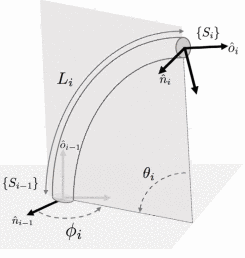
\includegraphics[width=0.5\textwidth]{graphics/oldparam.png}\
    \caption{The standard or "old" state parametrization. \imgcite{katzschmann_dynamic_2019}}
    \label{oldparam}
\end{figure}

The issue with this parametrization--which was mentioned in our discussion of the previous model--is that for a given physical configuration, it does not \textit{uniquely} map to a vector $\alpha_i$. In the case of the straight configuration for example, this means there are infinite choices of $\phi_i$ for $\theta_i=0$. Giving rise to the kinematic singularity mentioned previously.

Now in \cite{della_santina_improved_2020}, Della Santina et al. refers to the alternative state parametrization they propose as the "$q$-parametrization". \autoref{altparam} illustrates how the $i$-th segment of a PCC soft robot is now represented instead.

\begin{figure}[h!]
    \centering
    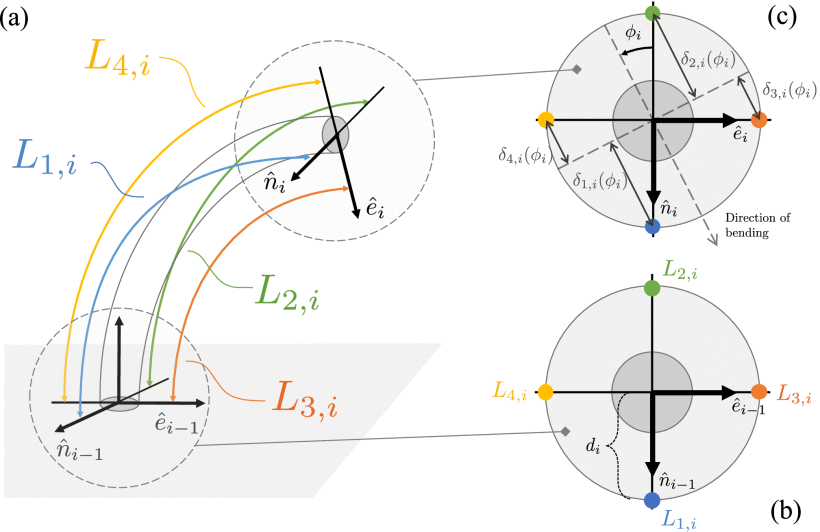
\includegraphics[width=0.5\textwidth]{graphics/altparam.png}
    \caption{The alternative "Arc-Length Parametrization". \imgcite{della_santina_improved_2020}}
    \label{altparam}
\end{figure}

This new "Arc-Length Parametrization" defines a configuration $q_i$ as $q_i = [\Delta_{x,i}, \Delta_{y,i}, \delta L_i]^T \in \mathbb{R}^3$. While explicit definitions of $\Delta_{x,i}$ and $\Delta_{y,i}$ will not be reported in this proposal, these two parameters essentially describe the difference in length between the two arcs whose ends are connected to the $\hat{n}$ (blue and green arcs) and $\hat{e}$ (yellow and orange arcs) axes, respectively.

With \cite{della_santina_improved_2020} proving that the $q$-parametrization is able to solve the limitations of the $\alpha$-parametrization, its kinematic robustness does make this model a great option to move forward with for this proposed thesis.        